\documentclass[12pt, letterpaper]{article}
\usepackage[utf8]{inputenc}
\usepackage{graphicx}
\usepackage{floatrow}

\usepackage[margin=2cm]{geometry} 



\renewcommand*\contentsname{Indholdsfortegnelse}


\begin{document}

\begin{titlepage}

\newcommand{\HRule}{\rule{\linewidth}{0.5mm}} % Defines a new command for the horizontal lines, change thickness here

\center % Center everything on the page
 
%----------------------------------------------------------------------------------------
%	HEADING SECTIONS
%----------------------------------------------------------------------------------------

\textsc{\LARGE Aarhus universitet}\\[1.5cm] % Name of your university/college
\textsc{\Large DSB}\\[0.5cm] % Major heading such as course name
\textsc{\large Semester 3}\\[0.5cm] % Minor heading such as course title

%----------------------------------------------------------------------------------------
%	TITLE SECTION
%----------------------------------------------------------------------------------------

\HRule \\[0.4cm]
{ \huge \bfseries Mini-projekt - Del 3}\\[0.4cm] % Title of your document
\HRule \\[1.5cm]
 
%----------------------------------------------------------------------------------------
%	AUTHOR SECTION
%----------------------------------------------------------------------------------------

% If you don't want a supervisor, uncomment the two lines below and remove the section above
\Large \emph{Studerende:}\\[1cm]
Mette \textsc{Hammer Nielsen-Kudsk - Studienr: 201408391}\\[0,5cm] % Your name
Martin \textsc{Banasik - Studienr: 201408398}\\[0,5cm] % Your name
Finja \textsc{Jette Ralfs - Studienr: 201303659}\\[0,5cm] % Your name
%----------------------------------------------------------------------------------------
%	DATE SECTION
%----------------------------------------------------------------------------------------

{\large November 15, 2015}\\[1,2cm] % Date, change the \today to a set date if you want to be precise

%----------------------------------------------------------------------------------------
%	LOGO SECTION
%----------------------------------------------------------------------------------------


\includegraphics[scale=0.5]{billeder/au}\\ % Include a department/university logo - this will require the graphicx package
 
 %\includegraphics[width=0.6\textwidth]{figurer/ASE}~\\[1cm]
%----------------------------------------------------------------------------------------

\vfill % Fill the rest of the page with whitespace


\end{titlepage}

\tableofcontents
\newpage

\newpage

\section{FIR - Finite impulse response}

En vægtet sum (udglatning, midling), som kører hen over input-signalet x(n). 

Differensligning for FIR-filteret og definition: 
$$ y(n)= \sum\limits_{k=0}^{M-1} b_k * x(n-k)$$

hvor, 
$$ x(n) = input $$
$$ y(n) = output $$
$$ b_k = filterets koefficienter $$ 
$$ M = filterets længde $$
$$ M-1 = filterets orden $$

\begin{figure}[!h]
           \begin{floatrow}
             \ffigbox{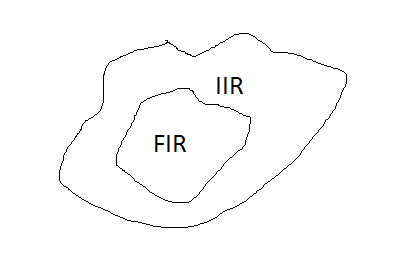
\includegraphics[width=1.1\linewidth]{billeder/domane}}		   			{\caption{FIR filter hører under IIR.}}
           \end{floatrow}
\end{figure}

Ved brugen af et FIR filter stopper outputtet. 


\section{IIR - Infinite impulse response}

IIR er en anden type for et digitalt filter, der kan have et uendeligt respons på en impuls. 

Differensligning for FIR-filteret og definition: 
$$ y(n)= \sum\limits_{k=0}^{M} b_k * x(n-k) - \sum\limits_{k=1}^{N}*a_k *y(n-k) $$
hvor, 
$$ x(n) = input $$
$$ y(n) = output $$
$$ b_k = filterets feedforward koefficienter $$ 
$$ M = filterets orden $$
$$ a_k = filterets feedback koefficienter $$

Ved brugen af et IIR filter stopper outputtet aldrig. 


\section{Z-transformation}

\begin{figure}[!h]
           \begin{floatrow}
             \ffigbox{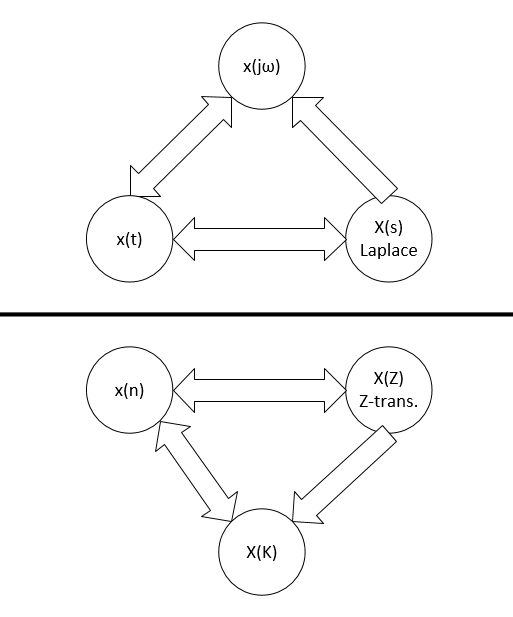
\includegraphics[width=1.1\linewidth]{billeder/trans}}		   			{\caption{Transformationer.}}
           \end{floatrow}
\end{figure}


Når vi snakker IIR filtre, så kan disse ofte være meget forvirrende, og det kan derfor være svært at se om filteret er stabilt eller ustabilt. Her indføres derfor z-transformation. 
Definition: 
$$ X(z)= \sum\limits_{n=0}^{M} x(n)*z^{-1}$$
Der er nogle forskellige ting, der er vigtige at vide ved z-transformation: 
$$\delta(n)$$
$$ z{\{\delta(n)}\}=1$$

Hvad ville der sker hvis impulsen er delayed? 
$$\delta(n-1)$$
$$ z{\{\delta(n-1)}\}=z^{-1}$$
$z^{-1}$ kaldes for unit delay. 

Vi kender, fra Analoge signal, til overføringsfunktioner. Det samme gælder her: 

$$ H(z)= \frac{output}{input} = \frac{Y(z)}{X(z)}$$

Når vi har fået lavet vores z-transformation kan vi altså finde overføringsfunktionen for filteret. 
Igennem overføringsfunktionen kan vi, i tælleren find ud af om filteret har nogle nulpunkter og i nævneren finde polerne. 
Hvis IIR filteret har 1 pol er det et 1. ordens IIR filter, hvis der havde været 2 poler, havde filteret været et 2. ordens IIR filter. Det er altså derfor nævneren, i overføringsfunktionen, hvor man kan finde polerne, der er interessant. Man kan herudfra se om filteret er stabilt eller ej. Hvis polerne er under eller lig 1 er filteret stabilt, hvis polerne er over 1 er filteret ustabilt. 
Da FIR filter altid er stabile, giver det ingen mening at lave z-transformation på disse. 


\section{Foldning}
Hvis vi ønsker at koble flere filter sammen, benytter vi kobling. 

Definition: 

$$ y(n)= \sum\limits_{k=0}^{M-1} h(k) * x(n-k) $$ \\

I MatLab benytter vi, ved foldning, funktionen "conv". 
Hvis vi har to signaler vi vil have koblet sammen, så repræsenteres dette ved en stjerne: 

\begin{center}
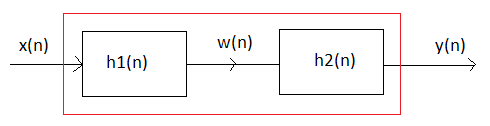
\includegraphics[width=0.7\textwidth]{billeder/foldning}
\end{center}

Den røde firkant omkredser de to signaler, der bliver foldet sammen. 

$$ h_1(n)\star h_2(n) $$


\section{Impulsfunktion: $\delta(n)$}


\section{Vindues metoden}
Når vi analytisk skal designe et filter, benytter vi os af vinduesmetoden. Her befinder vi os i frekvensverden (DFT). 
1) Vi specificer det ønskede frekvens karakteristik.
2) Herefter laver vi Invers DFT (IDFT). 
3) Så ganger vi vinduet på. 
4) Til sidst tjekker vi frekvenskarakteristik med DFT. 
 
\section{Filter design i MatLab}
Vi benytter os af to forskellige funktioner "fir1" og "fir2". 

- "fir1": 
$$ b = fir1(N, \frac{f_C}{0,5*f_s}, 'high') $$ 
hvor, 
$$ f_C = knækfrekvensen $$
$$ f_s = samplesfrekvens $$

Her vil MatLab lave et højpas filter, da vi har indskrevet 'high'. 
Hvis vi ønskede et lavpas filter skulle vi ikke havde skrevet noget. Ønskede vi et båndpas filter, ville vi skulle skrive bandpas og ved båndstop filer, bandstop. 

- "fir2": 
$$ b = fir2(N, ..., ...) $$
Her skal der indsættes amplituder. Benyt "help" funktionen i MatLab foran "fir2", hvis der ønskes mere information om denne funktion. 

Vi har i løbet af skriveprocessen lært at benytte funktionen "fdatool". Den er blevet brugt i løbet af dette miniprojekt til at designe et FIR lavpas filter og et FIR båndstop filter. 

\begin{figure}[!h]
           \begin{floatrow}
             \ffigbox{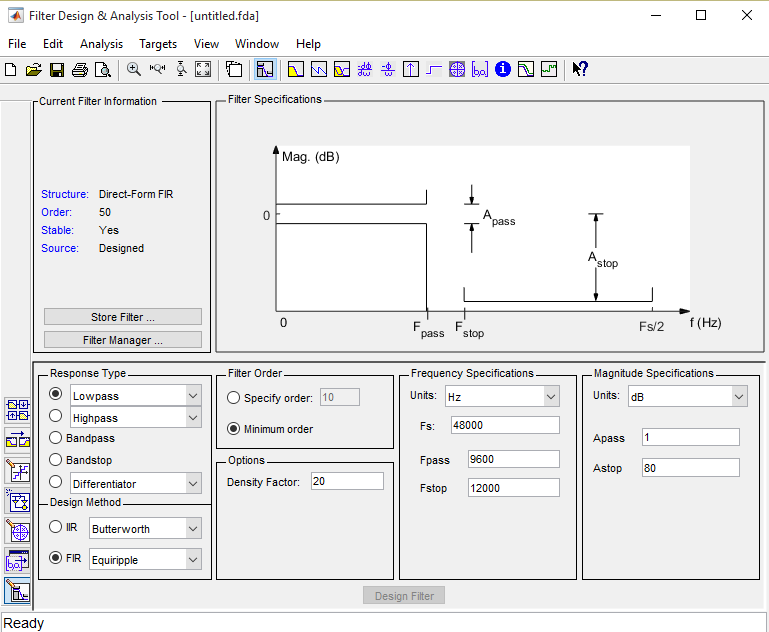
\includegraphics[width=1.1\linewidth]{billeder/fdatool}}		   			{\caption{fdatool i MatLab}}
           \end{floatrow}
\end{figure}



\section{Filtrering af EKG signal}

Der er blevet fundet et støjfyldt EKG-signal inde på siden Physionet. Her er EKG-signalet vist og som man kan se er der utrolig meget støj lige ved de 50 Hz. Det kan ses i tidsdomænet at EKG-signalet er ret støjfyldt efter hvert pulsslag, mellem PR-segmenterne og QT-segmenterne. Det ønsker vi fjernet. 

\begin{figure}[H]
           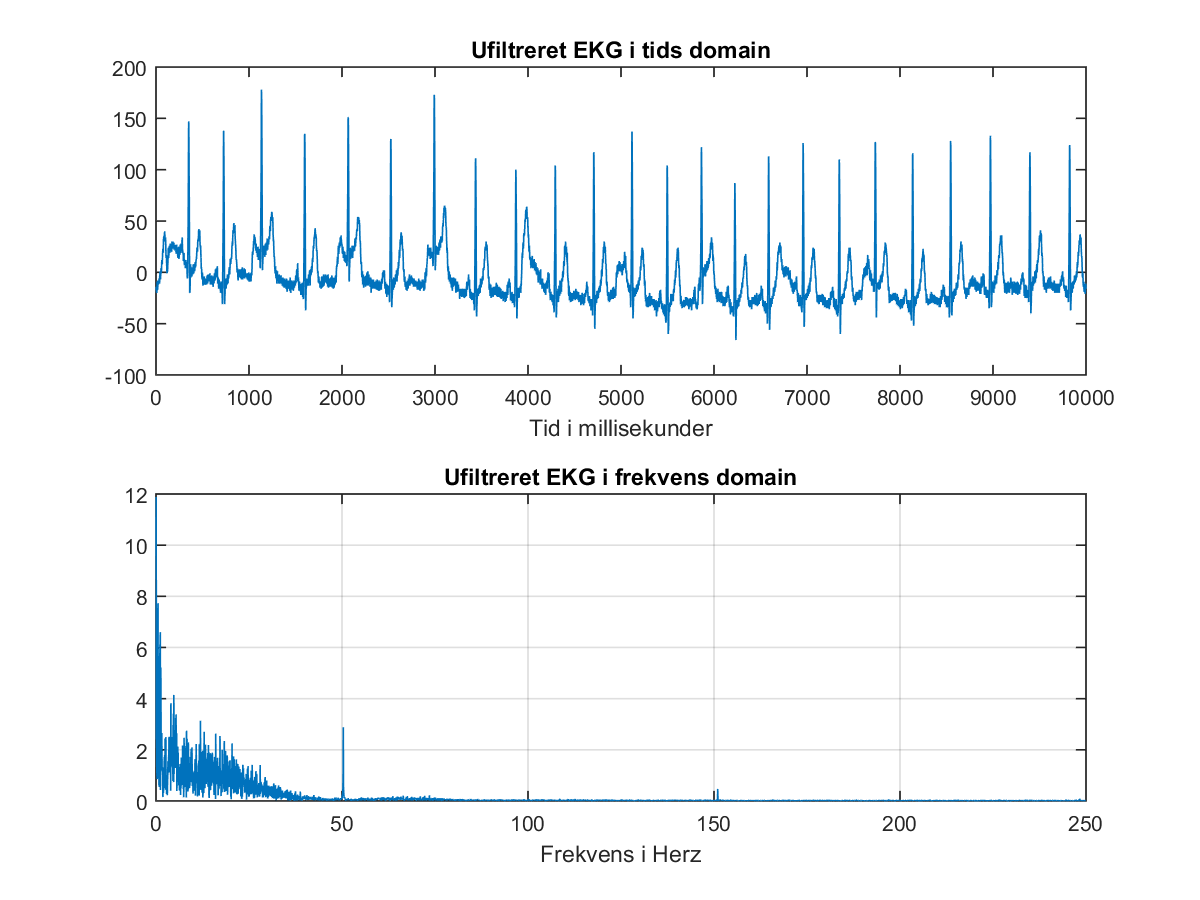
\includegraphics[width=\linewidth]{billeder/EKGufiltreret}	   							\caption{EKG ufiltreret.}
\end{figure}

Det mest iøjnefaldende er støjen ved de 50 Hz, så dem starter vi med at få fjernet. Det gøres i form af et IIR båndstopfilter. Det bliver designet vha. af MatLab funktionen "fdatool". Her indtastes:
$$ Fs = 500 $$
$$ Fpass1 = 47 $$
$$ Fstop1 = 48 $$
$$ Fstop2 = 52 $$
$$ Fpass2 = 53 $$

Vi har altså ønsket en knækfrekvens på de 50 Hz. 
Filteret loades herefter ind i MatLab filen og ligges ovenpå det støjfyldte EKG-signal i frekvensdomænet. 
Det kan nu ses på figurerne herunder at støjen ved de 50 Hz er blevet fjernet. Hvis vi sammenligner figur 3 og 4 i tidsdomænet kan det ses at støjen mellem de forskellige segmenter er mindsket. Det samme gælder i frekvensdomænet, hvor der i figur 3, kan ses støjen ved de 50 Hz - den er væk i figur 4 efter vi har kørt EKG-signalet igennem båndstop filteret.  
Hvis man kigger godt efter på frekvensdomænet i figur 4, kan man se lidt støj mellem 35 og 85 Hz. Det ønsker vi også fjernet. 

\begin{figure}[H]
           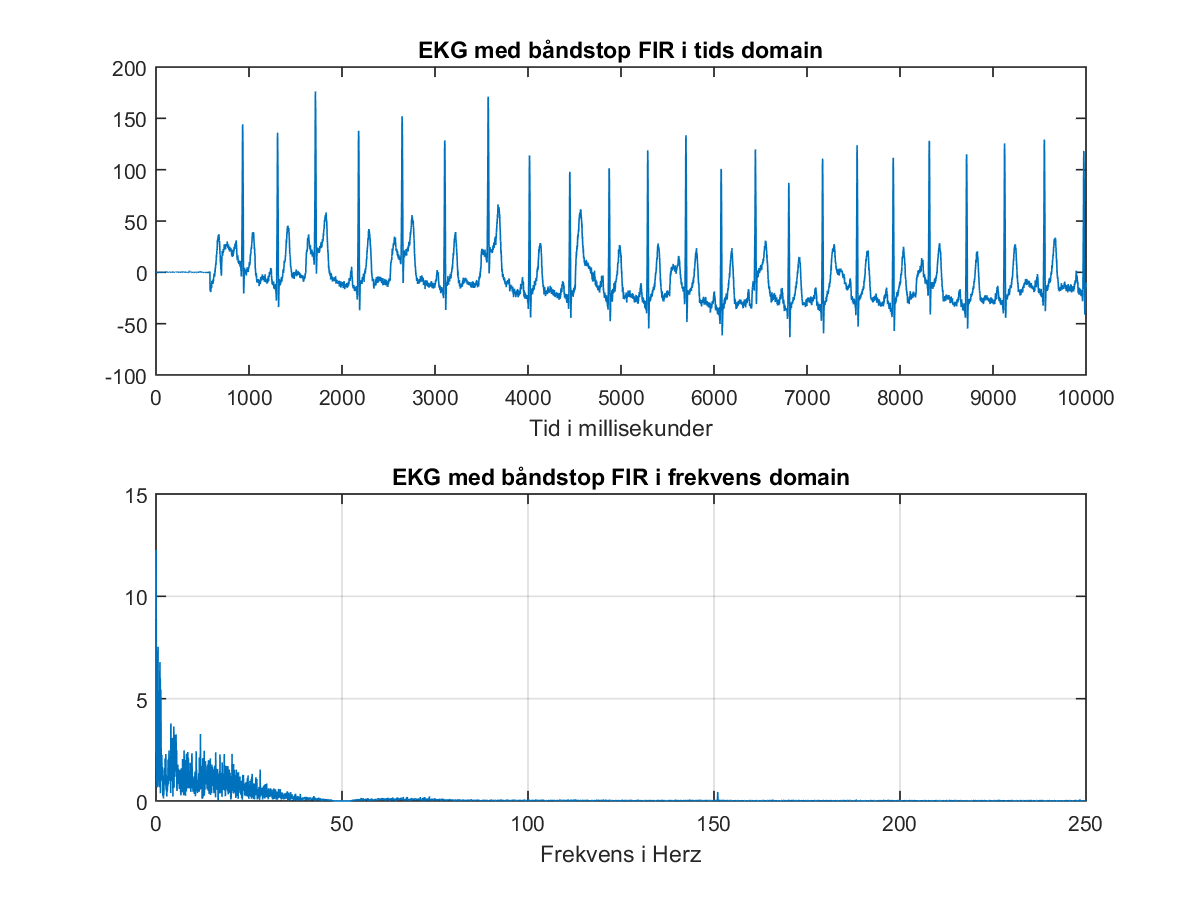
\includegraphics[width=\linewidth]{billeder/EKGstopbandFIR}	   							\caption{EKG med båndstop FIR.}
\end{figure}

Dette fjernes med et FIR lavpasfilter, der også bliver designet vha. "fdatool". Her indtastes: 

$$ Fs = 500 $$
$$ Fpass = 35 $$
$$ Fstop = 40 $$

Vi har altså ønsket en knækfrekvens på 38 Hz. 
Hvis man kigger på figur 5 og sammenligner med figur 4, kan man nu se i frekvensdomænet, at støjen efter de 35 Hz er blevet fjernet.
Igen kan vi se i tidsdomænet at vores EKG-signal er blevet meget pænere og mindre støjfyldt. Hvis vi går helt tilbage og sammenligner figur 3 og 5, kan vi se at EKG-signalet er meget pænere. 


\begin{figure}[H]
           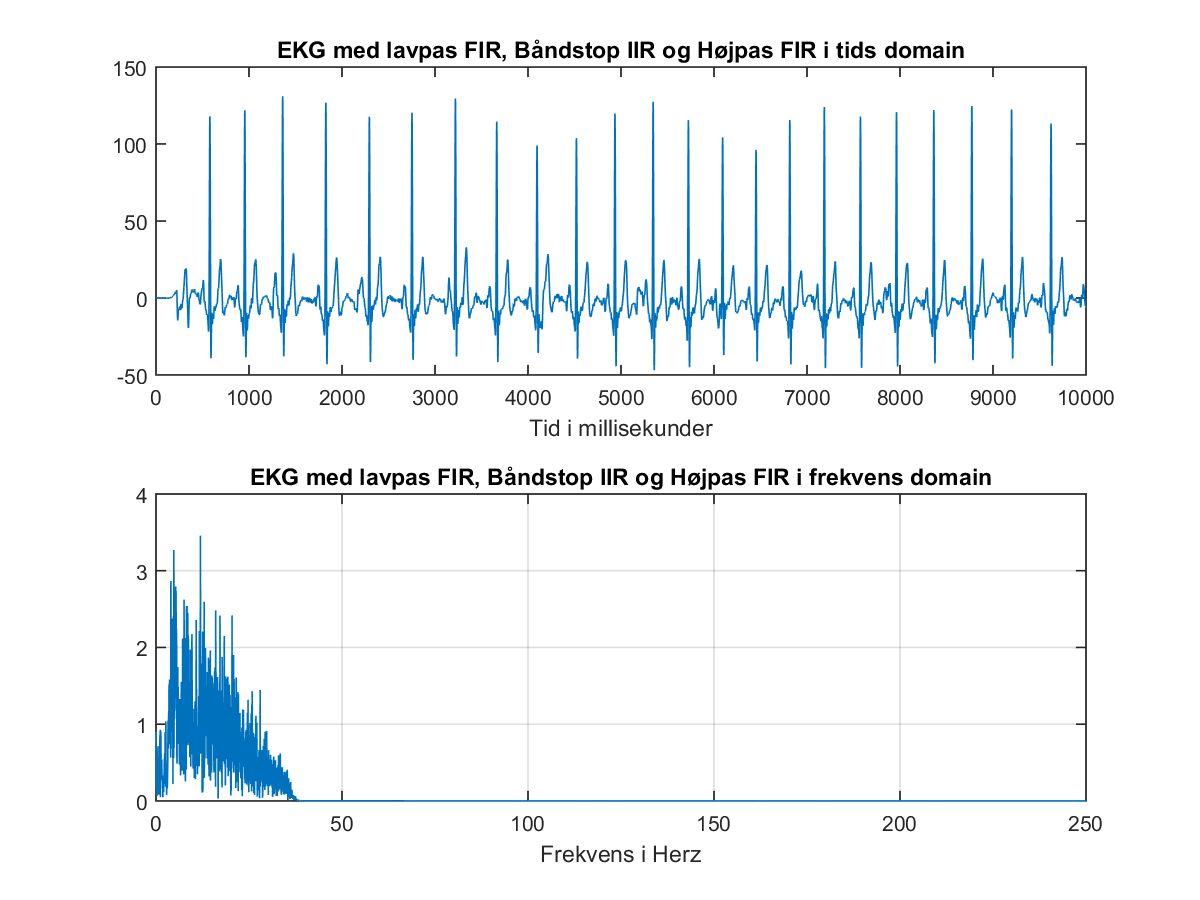
\includegraphics[width=\linewidth]{billeder/EKGlavpasFIR}	   							\caption{EKG med lavpas FIR.}
\end{figure}

For lettere at se forbedringerne har vi sat forbedringerne under hinanden vha. funktionen "subplot". Her har vi først EKG-signalet i tidsdomænet, hvor man tydeligt kan se at støjen er blevet fjernet. 

\begin{figure}[H]
           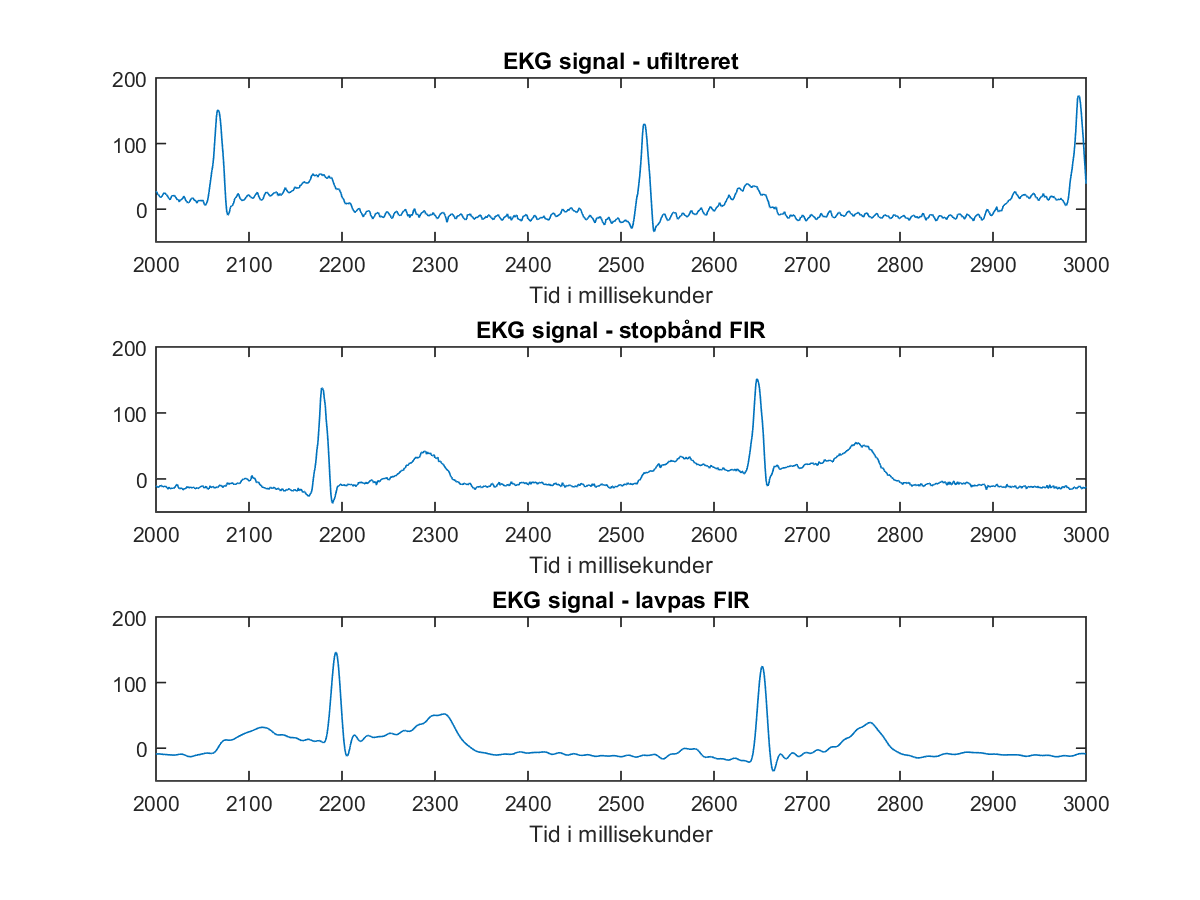
\includegraphics[width=\linewidth]{billeder/EKGtidsdomain}	   							\caption{Sammenligning af EKG i tidsdomæne.}
\end{figure}

Her har vi sammenligningen af signalerne i frekvensdomænet. Ved det ufiltreret EKG-signal ser vi tydeligt støjen ved de 50 Hz. Dem fik vi fjernet vha. båndstop filteret. 
Hvis man kigger godt efter kan man faktisk også se lidt støj ved 150 Hz. Da vi ønskede at fjerne støj fra 35 Hz og frem, så fik vi også fjernet støjen ved de 150 Hz. 


\begin{figure}[H]
           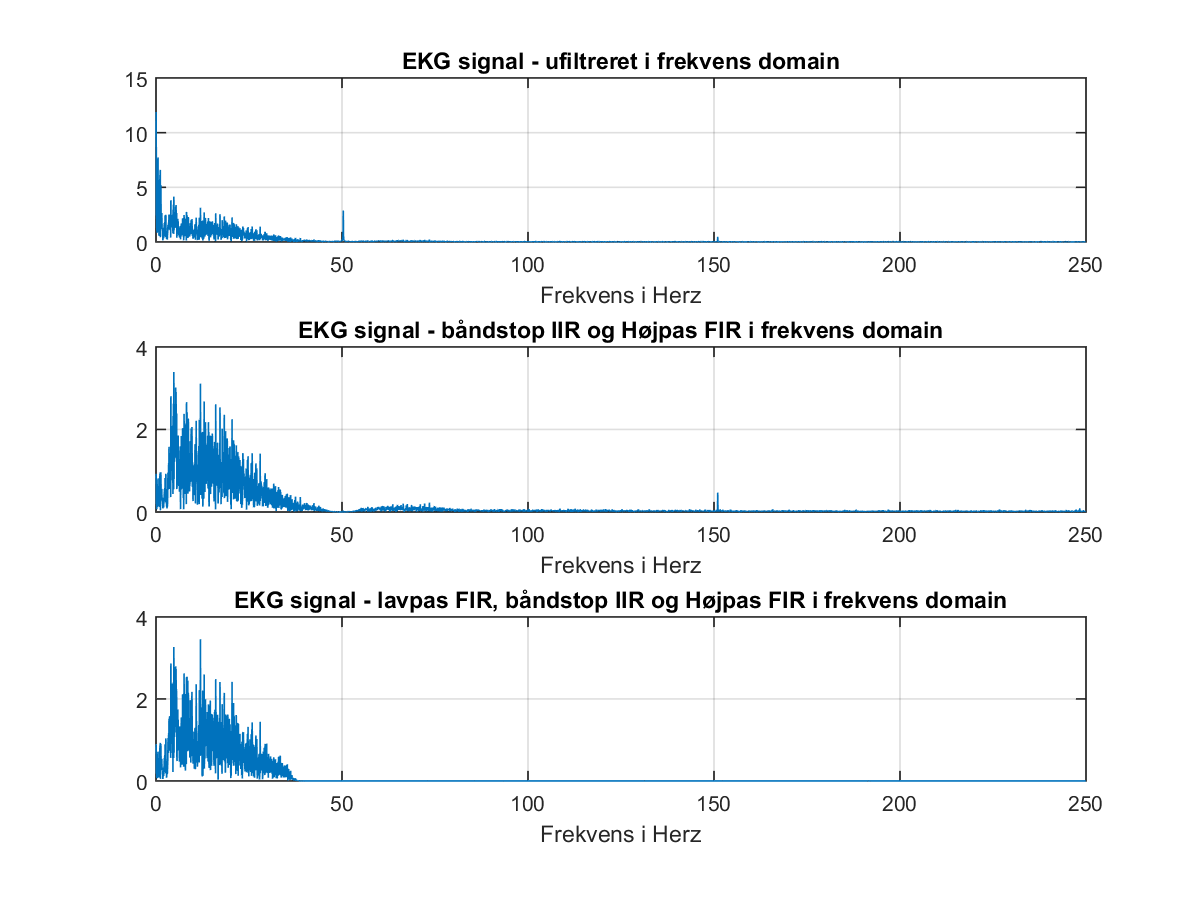
\includegraphics[width=\linewidth]{billeder/EKGfrekvensdomain}	   							\caption{Sammenligning af EKG i frekvensdomænet.}
\end{figure}


\section{Fremtidigt arbejde}
Vi ønsker at få lidt bedre styr på FIR og IIR filtre og hvordan de helt prævis hænger sammen. Vi har fået en god forståelse af hvad de gør, men vil alle gerne vide mere. Dette undersøges til næste miniprojekt og er derved vores fremtidige arbejde.

\section{Konklusion}
Vi kan konkludere at funktionen "fdatool" er super lækker at benytte når man skal have designet et filter. Man slipper for at bøvle med at skrive selve koden og hvordan MatLab funktionerne som f.eks. "fir1 og fir2" skal opbygges. Selvfølgelig skal man stadig kende fs og fc osv. men det giver jo sig selv. 
Vi har fået et klart større indblik i hvad de forskellige filtre kan, også ift. IIR og FIR filtre. Det giver meget bedre mening nu, efter man har siddet og leget med det og forsøgt sig frem med de forskellige filtre. Man har kunne se hvad virker på hvad og hvad helt sikkert ikke fungerer. 



\end{document}